\documentclass[11pt,a4paper]{article}

% ---------------------------------------------------------------------------
% Packages
% ---------------------------------------------------------------------------
\usepackage[utf8]{inputenc}
\usepackage[T1]{fontenc}
\usepackage{amsmath,amssymb}
\usepackage{graphicx}
\usepackage{booktabs}
\usepackage{geometry}
\usepackage{hyperref}
\usepackage{siunitx}
\usepackage{caption}
\usepackage{authblk}

\geometry{margin=2.5cm}
\hypersetup{colorlinks=true, linkcolor=blue, citecolor=blue, urlcolor=blue}

\sisetup{detect-all=true}

% ---------------------------------------------------------------------------
% Title / authors
% ---------------------------------------------------------------------------
\title{\textbf{Accounting for Material Plasticity to Reduce Displacement-Controlled Moments in Piping Stress Analysis: \\
The RCC-MRx Abatement Coefficient}}

\author[1]{Farid Tata}
\author[2]{Ir\'en\'ee Cornaton}
\author[2]{Thuy Pham}
\affil[1]{DAES}
\affil[2]{Octave}

\date{Pipe Stress Day, Lyon, France --- 28 May 2026}

\begin{document}

\maketitle

\begin{abstract}
Displacement-controlled (secondary) loads in nuclear piping systems are conventionally treated as self-limiting and are consequently penalised less severely than primary loads. The RCC-MRx code formalises this distinction through the \emph{elastic follow-up factor} $r_M$ and the associated \emph{abatement coefficient} $g$, which allow the displacement-dependent moment to be reduced when elasto-plastic behaviour of the material is properly accounted for. This paper revisits the theoretical basis of the elastic follow-up phenomenon --- as introduced by R.~Roche --- and benchmarks the RCC-MRx analytical procedure (RB~3643 and RB~3651) against a full elasto-plastic finite-element analysis of a simple elbow-and-straight-pipe test case. The elastic model is first calibrated between a beam-based piping code (Aspect Nuclear Pipe Stress, ``NS'' solver) and a shell finite-element model (MSC~Marc), matching the anchor reaction moment via the elbow flexibility factor $k$. An elasto-plastic shell analysis is then performed using a Ramberg--Osgood constitutive law representative of 316L(N) stainless steel at \SI{550}{\celsius}. The abatement coefficient computed from the RCC-MRx analytical route is compared with the coefficient back-calculated from the elasto-plastic Von Mises stress at the critical section. The comparison shows that the RCC-MRx coefficient ($g \approx 0.323$) is markedly less conservative than the value implied by the elasto-plastic reference calculation ($g \approx 0.436$), and that the associated primary-equivalent stress ($\sigma_{m}+\sigma_{b}=\SI{66.5}{MPa}$) underestimates the actual elasto-plastic Von Mises stress (\SI{86.5}{MPa}). Two candidate explanations are examined: (i) the code-prescribed conversion of the abated secondary stress into an equivalent primary stress, which reintroduces a conservatism factor of about 2.08 once compared on a consistent primary-stress basis; and (ii) the sensitivity of the elasto-plastic reference solution itself to the shell mesh density used to resolve elbow ovalisation. The paper closes with a discussion of the limitations of the Ramberg--Osgood representation across the operating temperature range and of the perspectives for including internal pressure in future work.
\end{abstract}

\tableofcontents

% =============================================================================
\section{Introduction}
% =============================================================================

Piping stress analysis distinguishes between \emph{primary} loads (pressure, weight, seismic inertia, etc.), which are not self-limiting and can lead to unbounded deformation if the material yields, and \emph{secondary} (displacement-controlled) loads, such as thermal expansion, which are self-limiting: once the material yields locally, the associated stresses relax and the deformation compatibility is preserved elastically or elasto-plastically by the remainder of the structure. Design codes therefore allow secondary stresses to be evaluated with more permissive criteria than primary stresses, provided the self-limiting character of the load is correctly represented.

The RCC-MRx code for high-temperature nuclear components formalises this distinction through the concept of the \emph{abatement coefficient} $g$ (RB~3651), which reduces the displacement-dependent moment used in the primary-type damage assessment. The coefficient $g$ is itself derived from the \emph{elastic follow-up factor} $r_M$ (RB~3643), a structural indicator of how much a locally yielding cross-section is elastically restrained (``followed up'') by the surrounding, comparatively stiffer, structure.

The objective of this work is twofold:
\begin{enumerate}
    \item to present, in a self-contained manner, the historical and theoretical background that leads from classical beam theory to the modern treatment of elastic follow-up and the abatement coefficient in RCC-MRx;
    \item to benchmark the RCC-MRx analytical procedure against a reference elasto-plastic finite-element (FE) shell analysis on a simple, well-defined elbow test case, in order to quantify how conservative (or non-conservative) the code procedure is with respect to a full non-linear reference solution.
\end{enumerate}

% =============================================================================
\section{Historical background}
% =============================================================================

The treatment of piping flexibility and secondary stresses has evolved over more than two and a half centuries, from the classical beam theories of the 18th century to the elasto-plastic follow-up concepts introduced in the 1980s. Table~\ref{tab:history} summarises the main milestones relevant to the present work.

\begin{table}[h]
\centering
\caption{Historical milestones in beam theory and piping flexibility analysis.}
\label{tab:history}
\begin{tabular}{@{}p{2.2cm}p{12.5cm}@{}}
\toprule
\textbf{Period} & \textbf{Contribution} \\
\midrule
1750 & Euler--Bernoulli beam theory: classical elastic bending equations. \\
1911 & Von~K\'arm\'an's work on the ovalisation of curved thin-walled tubes under bending \cite{VonKarman1911}: first bend flexibility factors. \\
$\sim$1920 & Timoshenko beam theory: shear deformation is included. \\
1940 & Development of flexibility calculations for high-temperature steam piping (up to \SI{650}{\celsius}) using graphical methods (Z-, L- and U-bend layouts). \\
Late 1940s--1950s & A.R.C.~Markl's fatigue testing programme on piping components (Tube Turns) \cite{Markl1955}: derivation of Stress Intensification Factors (SIFs) and generalisation of the flexibility-factor concept (building on von~K\'arm\'an); this work forms the modern basis of piping flexibility and fatigue analysis. \\
$\sim$1980 & R.~Roche introduces the concept of elastic follow-up and of plasticity effects into piping flexibility calculations \cite{Roche1987,MillardRoche1981}. \\
\bottomrule
\end{tabular}
\end{table}

\begin{figure}[h]
\centering
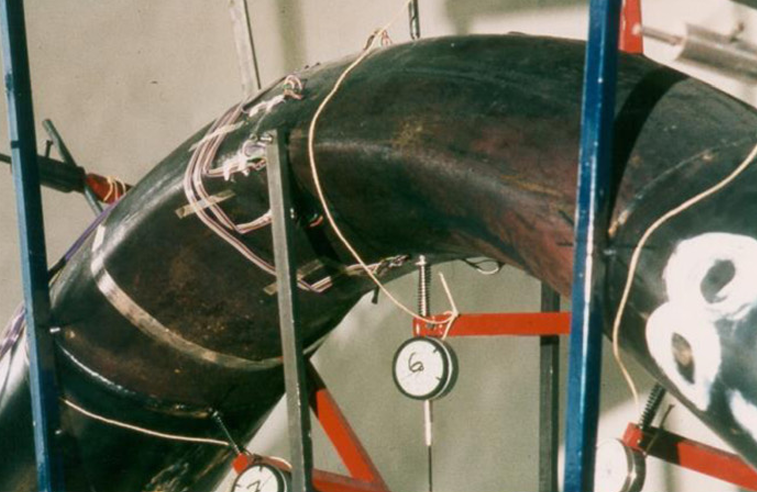
\includegraphics[width=0.55\textwidth]{figures/markl_fatigue_test_photo.png}
\caption{Photograph of one of A.R.C.~Markl's original fatigue test rigs (Tube Turns, late 1940s--1950s), showing a pipe elbow specimen instrumented with dial gauges under cyclic bending \cite{Markl1955}.}
\label{fig:markl-photo}
\end{figure}

\begin{figure}[h]
\centering
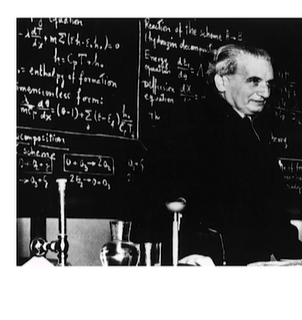
\includegraphics[width=0.4\textwidth]{figures/historical_lecture_photo.png}
\caption{A lecturer at the blackboard, illustrating the enthalpy/reaction-scheme formalism typical of the mid-20th-century engineering-science teaching from which the beam-theory and thermodynamic energy-balance concepts used throughout this paper are inherited.}
\label{fig:historical-lecture}
\end{figure}

% =============================================================================
\section{Beam theory and flexibility of curved pipes}
% =============================================================================

\subsection{Euler--Bernoulli and Timoshenko beam models}

The classical Euler--Bernoulli hypothesis neglects transverse shear deformation and rotational inertia; it is only valid for slender members. The Timoshenko beam theory retains both transverse shear and all inertia terms and remains valid for stockier members as well. For in-plane bending of a beam in the $(x,z)$ plane with constant cross-section and material along the longitudinal axis, the governing equations differ by the inclusion of (i) the rotational inertia associated with bending, (ii) the transverse shear flexibility (Timoshenko hypothesis), and (iii) the coupling between rotational and translational inertia \cite{Flejou2024}. Standard nuclear piping codes rely on Timoshenko-type beam elements for the straight and curved segments of the model. The corresponding governing partial differential equation for the transverse displacement $w(x,t)$ of a Timoshenko beam, including rotational inertia and shear-rotation inertia coupling, reads:

\begin{figure}[h]
\centering
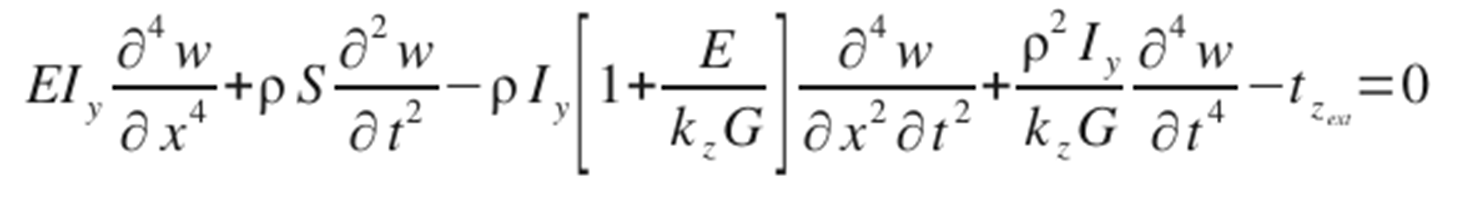
\includegraphics[width=0.85\textwidth]{figures/timoshenko_beam_equation.png}
\caption{Governing equation of the Timoshenko beam model for in-plane bending: $E$ is Young's modulus, $I_y$ the second moment of area, $\rho$ the mass density, $S$ the cross-sectional area, $k_z$ the shear correction factor, $G$ the shear modulus, and $t_{z_{ext}}$ the externally applied transverse load per unit length.}
\label{fig:timoshenko-eq}
\end{figure}

\subsection{Elbow ovalisation and flexibility factors}

Under in-plane bending, a curved pipe (elbow) undergoes cross-sectional \emph{ovalisation}: the circular cross-section distorts into an oval shape. This ovalisation increases the flexibility of the elbow well beyond the prediction of classical (straight) beam theory. The \emph{flexibility factor} $k$ is defined as the ratio between the rotation per unit length of the curved component and the rotation per unit length of an equivalent straight pipe under the same bending moment.

Following von~K\'arm\'an and Beskin's approximation \cite{VonKarman1911}, the flexibility factor of a smooth, unpressurised elbow can be written, to a good approximation, in terms of the non-dimensional flexibility characteristic $h$:
\begin{equation}
h = \frac{t\,R}{r^{2}}, \qquad k = \frac{1.65}{h} = \frac{1.65\, r^{2}}{t\,R},
\label{eq:flexfactor}
\end{equation}
where $t$ is the wall thickness, $r$ the mean cross-sectional radius, and $R$ the bend radius.

\begin{figure}[h]
\centering
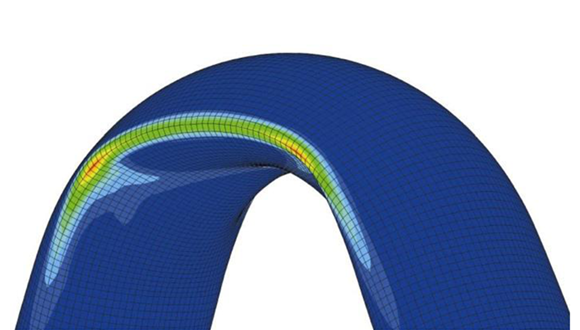
\includegraphics[width=0.5\textwidth]{figures/elbow_ovalisation_contour.png}
\caption{Finite-element illustration of elbow cross-section ovalisation under in-plane bending: the stress concentration follows the ovalised region at the crown of the bend.}
\label{fig:ovalisation}
\end{figure}

For the elbow considered in the benchmark of this paper (outer diameter $D=\SI{219.07}{mm}$, thickness $t=\SI{3.76}{mm}$, bend radius $R=\SI{500}{mm}$, hence $r = \tfrac12(D-t) = \SI{107.66}{mm}$), Eq.~\eqref{eq:flexfactor} gives $h=0.1622$ and $k=10.17$, in agreement with the value used in the benchmark (Section~\ref{sec:benchmark}).

\paragraph{Link with Stress Intensification Factors (SIFs).} Markl observed that the flexibility factor $k$ and the stress intensification factor $i$ (Section~\ref{sec:sif}) are governed by the same underlying physics --- the ovalisation of the cross-section --- and that the inaccuracies affecting $k$ and $i$ tend to compensate one another. This observation justifies the continued use of simple, closed-form expressions such as Eq.~\eqref{eq:flexfactor} in modern piping codes.

% =============================================================================
\section{Stress Intensification Factors and the Markl fatigue design curve}
\label{sec:sif}
% =============================================================================

Because of the geometric and material discontinuities near fittings, welds and bends, the local stress in these areas is amplified with respect to the nominal beam-theory stress. This amplification is expressed through the \emph{Stress Intensification Factor} (SIF), $i$. Following Markl's original definition, $i$ is not simply a stress concentration factor but a fatigue \emph{severity} factor: it quantifies how much the fatigue endurance of a given detail is degraded relative to a plain, defect-free straight pipe subjected to the same nominal bending stress.

Markl established an empirical fatigue ($S$--$N$) design curve from cyclic bending tests on straight, girth-welded pipe sections, of the form
\begin{equation}
S \cdot N^{n} = m ,
\label{eq:markl}
\end{equation}
where $S = iM/Z$ is the nominal bending stress amplitude multiplied by the SIF, $Z$ the section modulus, $N$ the number of cycles to failure, and $m$, $n$ empirical constants fitted from the test data (for austenitic stainless steels, $m \approx \SI{1940}{MPa}$ and $n \approx 0.2$).

A key methodological point made by Markl is the distinction between two possible references for the SIF:
\begin{itemize}
    \item a \emph{theoretical} reference, based on tests on ideal, notch-free homogeneous material, which yields comparatively high SIFs;
    \item the \emph{as-built product} reference, based on tests on actual commercial, girth-welded pipe (including realistic surface imperfections), which is the reference actually adopted by the design rules.
\end{itemize}
This choice of reference explains why SIFs measured in fatigue tests are systematically lower than those predicted by purely elastic (theoretical) stress-concentration analysis, and it underlies the overall internal consistency of Markl's approach.

% =============================================================================
\section{Elastic follow-up: from local (Neuber) to global (Roche) redistribution}
% =============================================================================

Two conceptually different, but often confused, corrections are used to relate an elastically computed stress or strain field to the actual elasto-plastic response of a structure: \emph{Neuber's rule} and the \emph{elastic follow-up effect}. Their essential differences are summarised in Table~\ref{tab:neuber-followup}.

\begin{table}[h]
\centering
\caption{Neuber local correction versus global elastic follow-up.}
\label{tab:neuber-followup}
\begin{tabular}{@{}lll@{}}
\toprule
 & \textbf{Neuber} & \textbf{Elastic follow-up} \\
\midrule
Nature & Local & Global \\
Affected zone & Notch / point & Whole structure \\
Type of phenomenon & Stress concentration & Strain redistribution \\
Role & Corrects a local stress peak & Corrects the overall structural response \\
\bottomrule
\end{tabular}
\end{table}

Elastic follow-up describes how a locally yielding (softening) section of a structure is ``followed up'' by the surrounding, stiffer parts, which continue to impose additional deformation on the yielded section because the imposed \emph{overall} displacement must still be accommodated. Depending on how stiff the surrounding structure is relative to the yielding section, the behaviour of that section under a nominally secondary (displacement-controlled) load can range from purely secondary (self-limiting, if the surrounding structure is very flexible and simply relaxes) to effectively primary (if the surrounding structure is very stiff and keeps imposing the full displacement onto the yielded, and therefore weaker, section).

\subsection{The Ramberg--Osgood constitutive law}

To model the elasto-plastic material response, the Ramberg--Osgood law is used, in the exact form used in the benchmark computations:
\begin{equation}
\varepsilon(\sigma) = \frac{\sigma}{E} + 0.01\left(\frac{\sigma}{C_0\,(R_{p0.2})_{\mathrm{mean}}}\right)^{1/n_0} \;\equiv\; \frac{\sigma}{E} + \left(\frac{\sigma}{K}\right)^{1/n_0}, \qquad K(T) = C_0\,R_{p0.2}(T),
\label{eq:RO}
\end{equation}
with, for 316L(N) stainless steel, $n_0 = 0.1125$ ($1/n_0 = 8.89$) and $C_0 = 1.198$; at the benchmark temperature of \SI{550}{\celsius}, $R_{p0.2} \approx \SI{106}{MPa}$, giving $K \approx \SI{131.8}{MPa}$. The strength coefficient $K(T)$ evolves with temperature through the temperature-dependent yield strength $R_{p0.2}(T)$, whereas $C_0$ and $n_0$ retain the same normalised curve shape at all temperatures --- i.e., no change of hardening \emph{shape} with temperature is assumed. A sensitivity study reported in the presentation, using an alternative parameter set ($C_0=1.233$, $n_0=0.130$, i.e. $1/n_0=7.69$, $K\approx\SI{135.6}{MPa}$) calibrated on the same \SI{550}{\celsius} tensile data, produces a stress--strain curve only marginally softer than the reference one (e.g. about \SI{2}{MPa} lower at $\varepsilon_t=2\%$), confirming that the choice of hardening parameters is not the dominant source of discrepancy discussed in Section~\ref{sec:discussion}.

Several open questions regarding the domain of validity of this simplified, temperature-invariant hardening shape are noted in the presentation (and are only partially addressed here): the sensitivity to strain rate, to monotonic versus cyclic hardening, to the number of cycles, and to environment (air, PWR primary water, sodium, etc.). For reference, an example comparison at $\SI{0.01}{}$ true strain shows a stress discrepancy of about \SI{4.0}{MPa} ($\sim$\SI{5}{\percent}) between candidate hardening curves \cite{NASAn1930}.

\subsection{Roche's spring-bar analogy}

R.~Roche's original demonstration of elastic follow-up \cite{Roche1987} uses a simple three-bar analogy:
\begin{itemize}
    \item \textbf{Bar 1} is subjected to a purely primary load: the elastically computed stress--strain state $(\sigma_{\mathrm{el}},\varepsilon_{\mathrm{el}})$ moves, once plasticity is included, to $(\sigma_1,\varepsilon_1)$ on the Ramberg--Osgood curve, following the classical, dangerous, primary-load behaviour (unbounded deformation for stresses above yield).
    \item \textbf{Bar 2} is subjected to a purely secondary (displacement-controlled) load: with plasticity, the elastic state $(\sigma_{\mathrm{el}},\varepsilon_{\mathrm{el}})$ moves to $(\sigma_2,\varepsilon_2)$, exhibiting the self-limiting character typical of secondary stresses.
    \item \textbf{Bar 3} reproduces Bar 2's geometry and loading but adds a \emph{spring} in series, with an imposed end displacement calibrated so that the resulting \emph{elastic} stress equals that of Bars 1 and 2. Despite representing a nominally purely secondary load case, Bar 3 exhibits an intermediate behaviour, between that of Bar 1 (primary) and Bar 2 (secondary): $(\sigma_3,\varepsilon_3)$ lies between $(\sigma_1,\varepsilon_1)$ and $(\sigma_2,\varepsilon_2)$.
\end{itemize}

This example demonstrates that a nominally secondary stress can, in the presence of elastic follow-up (represented here by the series spring), behave partly like a primary stress. A parametric study on the spring stiffness $k_2$ confirms this trend continuously: as $k_2 \to \infty$ (rigid spring), Bar 3's response tends towards Bar 2's purely secondary behaviour; as $k_2 \to 0$ (very soft spring), Bar 3's response tends towards Bar 1's purely primary behaviour. This is exactly the behaviour later formalised by RCC-MRx through the elastic follow-up factor $r_M$ and the abatement coefficient $g$ (Section~\ref{sec:rccmrx}).

\begin{figure}[h]
\centering
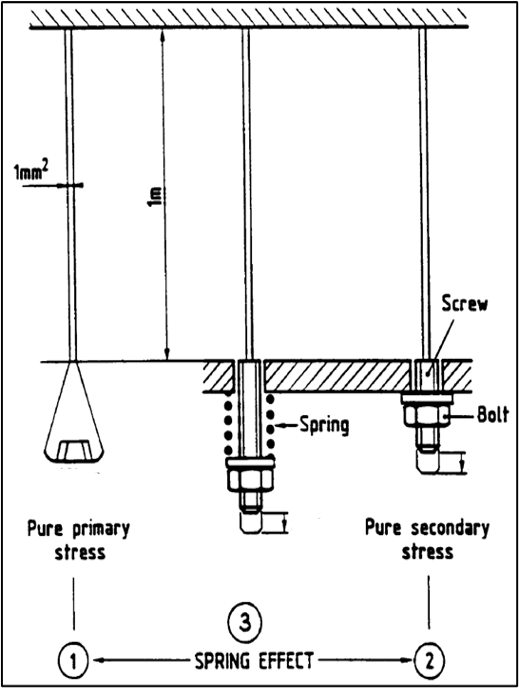
\includegraphics[width=0.45\textwidth]{figures/roche_spring_diagram_english.png}
\caption{Roche's original spring-bar analogy: Bar~1 (left) carries a pure primary stress (dead-weight-like load); Bar~2 (centre) carries a pure secondary stress through a soft spring; Bar~3 (right) reproduces the secondary loading through a bolted, effectively rigid connection, producing an intermediate, ``spring effect'' behaviour between Bars~1 and~2.}
\label{fig:roche-spring-diagram}
\end{figure}

A three-bar FE validation of this analogy, carried out with MSC~Marc on bars of unit cross-section, gives an elastic reference stress $\sigma_{\mathrm{el}}=\SI{126}{MPa}$; the elasto-plastic calculations give $\sigma_1=\SI{126.34}{MPa}$ for the purely primary Bar~1 (\emph{linear-primary} job) and $\sigma_2=\SI{82.3}{MPa}$ for the purely secondary Bar~2 (\emph{nonlinear-secondary-beam2} job). For Bar~3, a parametric study on the series-spring stiffness $k_2$ confirms the continuous transition announced above: the computed equivalent stress spans the range between $\sigma_2$ and $\sigma_1$ as $k_2$ increases, e.g. $\sigma_3 = \SI{90.3}{MPa}$ for a representative intermediate stiffness (Figure~\ref{fig:bar3-contour}), approaching $\sigma_1$ for stiffer springs and $\sigma_2$ for softer springs.

\begin{figure}[h]
\centering
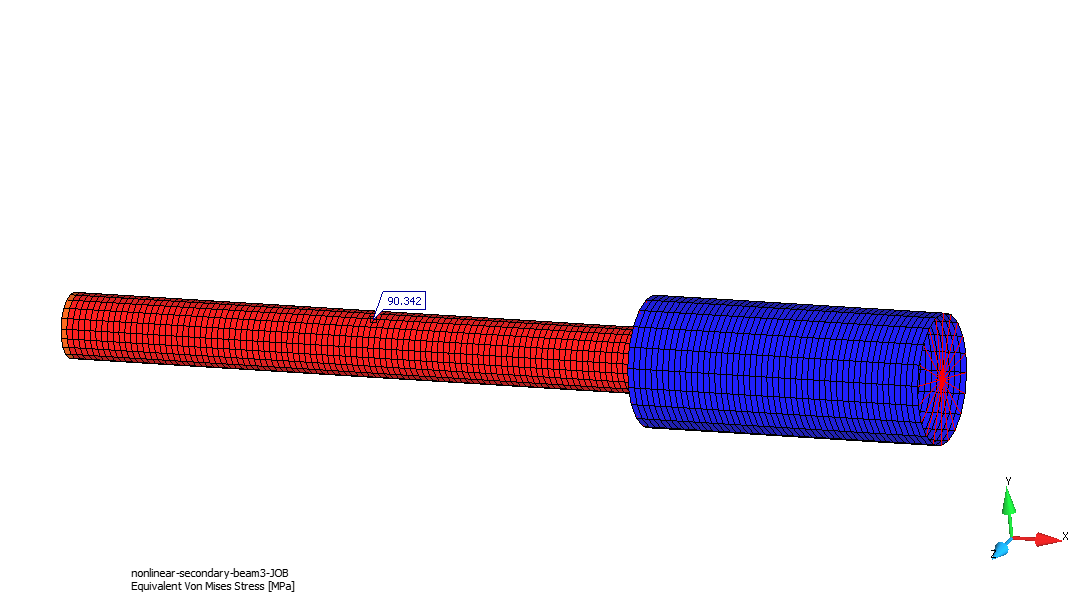
\includegraphics[width=0.7\textwidth]{figures/bar3_spring_vonmises.png}
\caption{MSC~Marc equivalent von~Mises stress contour for Bar~3 (\emph{nonlinear-secondary-beam3} job): the stress in the flexible segment reaches \SI{90.342}{MPa}, an intermediate value between Bar~1's primary stress ($\sigma_1=\SI{126.34}{MPa}$) and Bar~2's secondary stress ($\sigma_2=\SI{82.3}{MPa}$), illustrating the ``spring effect'' for a representative spring stiffness $k_2$.}
\label{fig:bar3-contour}
\end{figure}

\begin{figure}[h]
\centering
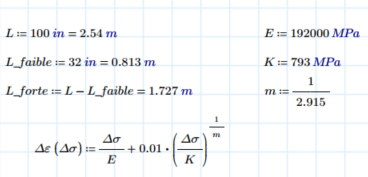
\includegraphics[width=0.55\textwidth]{figures/roche_example.png}
\caption{Numerical data from Roland Roche's original worked example (straight bar of total length $L=\SI{2.54}{m}$, split into a flexible segment $L_{\mathrm{faible}}=\SI{0.813}{m}$ and a stiff segment $L_{\mathrm{forte}}=\SI{1.727}{m}$, with $E=\SI{192000}{MPa}$, Ramberg--Osgood parameters $K=\SI{793}{MPa}$, $m=1/2.915$), illustrating the calculation of the elastic follow-up factor on a simple two-segment bar.}
\label{fig:roche-example}
\end{figure}

% =============================================================================
\section{The RCC-MRx elastic follow-up factor and abatement coefficient}
\label{sec:rccmrx}
% =============================================================================

\subsection{Energy balance and definition of $r_M$}

RCC-MRx clause RB~3643 formalises the elastic follow-up factor $r_M$ from an energy balance of the purely elastic calculation, following R.~Roche's original derivation (reproduced in full in Appendix~\ref{app:roche}). Let $(\sigma_{\mathrm{el}},\varepsilon_{\mathrm{el}})$ be the elastically computed equivalent stress and strain at the section of interest, and $(\sigma,\varepsilon)$ the actual (elasto-plastic) equivalent stress and strain reached at the same section once the true, non-linear material law (here, Ramberg--Osgood, Eq.~\eqref{eq:RO}) is accounted for, with the loading history assumed radially proportional ($\bar{\bar\sigma} = \varphi\,\bar{\bar\sigma}_0$, i.e. the elasto-plastic stress tensor field remains everywhere proportional to the elastic one through a single scalar $\varphi$). RCC-MRx defines the elastic follow-up factor as
\begin{equation}
r_M \;=\; \frac{E(\varepsilon-\varepsilon_{\mathrm{el}})}{\sigma-\sigma_{\mathrm{el}}} \Big/ (-1)\;=\;\frac{-E(\varepsilon-\varepsilon_{\mathrm{el}})}{\sigma-\sigma_{\mathrm{el}}} \;=\; \frac{T}{t}-1 \;\ge 0,
\label{eq:rM}
\end{equation}
where $t$ is the \emph{local} resilience (degree of elasticity) of the section under consideration, and $T$ is a \emph{global} resilience computed over the whole structure by weighting every section by its elastic reference stress:
\begin{equation}
T = \frac{\int \sigma_{\mathrm{ref}}^2 A\, ds}{\displaystyle\int \frac{\sigma_{\mathrm{ref}}^2 A}{t}\, ds}, \qquad
\frac{1}{t} = \frac{\varepsilon_{M,p}(\sigma_{\mathrm{ref}})}{\sigma_{\mathrm{ref}}/E}, \qquad
\sigma_{\mathrm{ref}}^2 = \left[0.79\,B_2\,\frac{(m)'_R}{Z}\right]^2 + \left[0.87\,\frac{m_1}{Z}\right]^2,
\label{eq:Tglobal}
\end{equation}
with $\varepsilon_{M,p}(\sigma) = \left[\sigma/\big(C_0\,(R_{p0.2})_{\mathrm{moy}}\big)\right]^{1/n_0}$ the plastic part of the mean Ramberg--Osgood curve (Eq.~\eqref{eq:RO}), and $m_1$, $(m)'_R$ the primary and secondary (resultant) moments at the section, $Z$ its section modulus. Equation~\eqref{eq:Tglobal} is the practical, piping-code form of $T$; its rigorous derivation from the energy balance $\iiint \bar{\bar\sigma}_0:\bar{\bar\varepsilon}\,dV = \iiint \bar{\bar\sigma}_0:\bar{\bar\varepsilon}_0\,dV$ is given in Appendix~\ref{app:roche}, Eqs.~(13)--(14) and (22).

For isotropic materials, the rigorous derivation of Appendix~\ref{app:roche} gives $r_M = \frac{2(1+\nu)}{3}\left(\frac{T}{t}-1\right)$, which for steels ($\nu=0.3$) gives $r_M = 0.867\left(\frac{T}{t}-1\right)$. In a conservative manner, RCC-MRx takes $\frac{2(1+\nu)}{3}\approx 1$ (absorbing the 3-D correction into a separate stress index of 0.87 applied to pressure and torsional moments), so that the code ultimately retains the simple form of Eq.~\eqref{eq:rM}, $r_M = T/t - 1$.

The factor $r_M$ has the following limiting behaviour:
\begin{itemize}
    \item $r_M = 0$ ($T=t$): no elastic follow-up; the stress is purely secondary (fully self-limiting).
    \item $r_M \to \infty$ ($T \gg t$): very significant elastic follow-up; the stress behaves as purely primary.
\end{itemize}
Note that a \emph{higher} $r_M$ is treated by the code as a \emph{more conservative}, more primary-like, assumption; taking $r_M(\mathrm{coeff}=1) > r_M(\mathrm{coeff}=0.867)$ is therefore itself a conservative simplification.

In the Roche three-bar analogy, Bar 2 (no spring) corresponds to $r_M=0$, Bar 1 (rigid connection) corresponds to $r_M\to\infty$, and Bar 3 (elastic spring) lies at an intermediate, finite value of $r_M$ that depends on the spring stiffness $k_2$.

\subsection{Abatement coefficient $g$}

For a section without internal pressure, RCC-MRx clause RB~3651.1131 (Figure ``RB~3651.1132: abatement coefficient $g$'' of the code, reproduced in Figure~\ref{fig:rccmrx-official}) defines the abatement coefficient as the ratio $g=\sigma/\sigma_{\mathrm{el}}$ of the true elasto-plastic stress to the elastically computed stress at the same imposed strain, which can be expressed directly from $r_M$ and the Ramberg--Osgood law as

\begin{figure}[h]
\centering
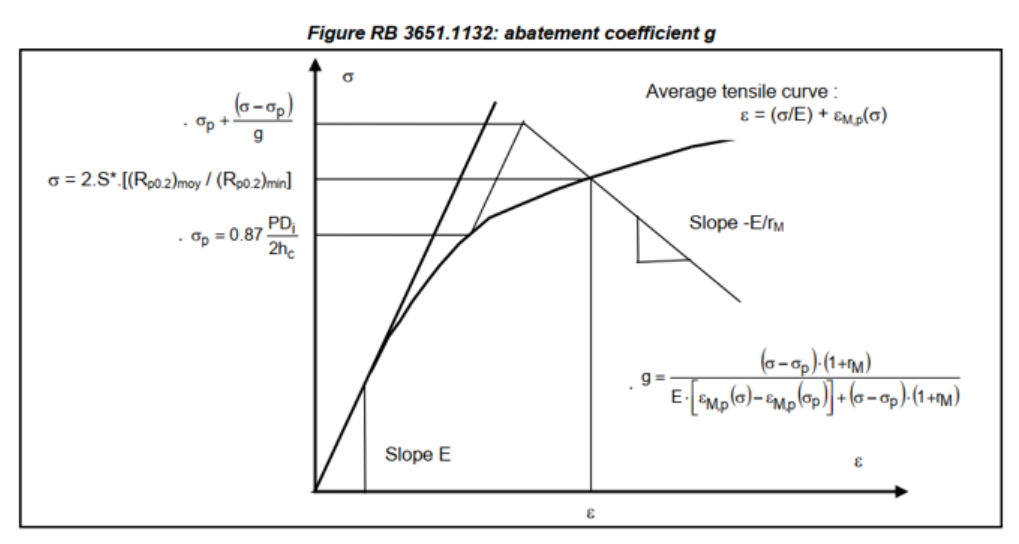
\includegraphics[width=0.8\textwidth]{figures/rccmrx_official_g_figure.png}
\caption{RCC-MRx Figure RB~3651.1132 (reproduced from the code): graphical definition of the abatement coefficient $g$, showing the average Ramberg--Osgood tensile curve, the elastic (slope $E$) and elastic-follow-up (slope $-E/r_M$) construction lines, the primary membrane stress $\sigma_p$ and allowable stress $S^{*}$.}
\label{fig:rccmrx-official}
\end{figure}
\begin{equation}
g \;=\; \frac{\sigma\,(1+r_M)}{E\,\varepsilon_{M,p}(\sigma) + \sigma\,(1+r_M)} .
\label{eq:gsimple}
\end{equation}
When a primary membrane stress from pressure, $\sigma_P = 0.87\,\dfrac{P D_i}{2h_c}$, is also present at the section (with $\sigma_P<\sigma$), the code generalises Eq.~\eqref{eq:gsimple} to
\begin{equation}
g \;=\; \frac{(\sigma-\sigma_P)(1+r_M)}{E\left[\varepsilon_{M,p}(\sigma)-\varepsilon_{M,p}(\sigma_P)\right] + (\sigma-\sigma_P)(1+r_M)} .
\label{eq:gfull}
\end{equation}
The coefficient $g$ is then used to reduce (``abate'') the displacement-dependent moment $M$ (secondary, in the classical sense) into an abated value $g\,m$, which is combined with the primary loads in the assessment of primary-type (P-type) damage through the RCC-MRx CMS1 stress-limitation rule (RB~3651.1131):
\begin{equation}
\overline{s_m+s_b} = \left[\left(D_1\left[\frac{PD_i}{2h_c}\right]\right)^2 + \left\langle D_2/Z,\, M + g\cdot m\right\rangle^2\right]^{0.5} \le S^{*} .
\label{eq:CMS1}
\end{equation}
In this way, the combined effects of elastic follow-up, plasticity and elasticity are accounted for in the P-type damage check of RCC-MRx, via $\overline{s_m+s_b}$, without requiring the analyst to perform a full elasto-plastic finite-element calculation.

This raises a natural verification question, addressed by the benchmark of this paper: \emph{is it necessary to explicitly reconsider secondary loads in the primary-stress validation, and if so, does the RCC-MRx analytical route ($r_M$, $g$) correctly and conservatively capture the elasto-plastic reality?}

% =============================================================================
\section{Benchmark description}
\label{sec:benchmark}
% =============================================================================

\subsection{Geometry, material and boundary conditions}

The benchmark model consists of a single elbow connecting two straight pipe runs, with fixed anchors at both ends:
\begin{itemize}
    \item Cross-section: outer diameter \SI{219.07}{mm}, wall thickness \SI{3.76}{mm};
    \item Straight lengths (nodes 10--20 and 30--40): \SI{2000}{mm} each;
    \item Elbow bend radius: \SI{500}{mm};
    \item Fixed anchors at end nodes 10 and 40;
    \item Thermal expansion loading from \SI{20}{\celsius} to \SI{550}{\celsius};
    \item No internal pressure;
    \item Material properties at \SI{550}{\celsius}: $E = \SI{155}{GPa}$, $\nu = 0.3$, $\alpha = 18.5\times 10^{-6}\,\si{\per\celsius}$, $R_{p0.2} \approx \SI{106}{MPa}$, Ramberg--Osgood parameters $n_0 = 0.1125$, $C_0 = 1.198$.
\end{itemize}

\begin{figure}[h]
\centering
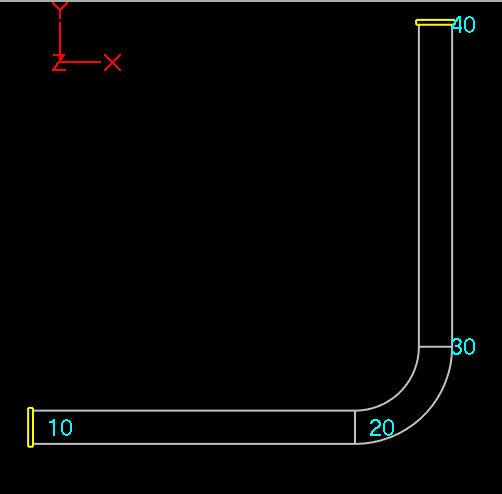
\includegraphics[width=0.45\textwidth]{figures/benchmark_geometry_nodes.png}
\caption{Benchmark geometry: elbow connecting two straight pipe runs, with fixed anchors at end nodes 10 and 40, and the elbow tangent points at nodes 20 and 30.}
\label{fig:benchmark-geometry}
\end{figure}

\subsection{Numerical models}

Two independent numerical models are used and cross-checked:
\begin{itemize}
    \item \textbf{Aspect Nuclear Pipe Stress} (``NS'' solver, PEPS~8.0), a beam-element piping-code model in which the elbow flexibility is represented through the analytical flexibility factor $k$ of Eq.~\eqref{eq:flexfactor};
    \item \textbf{MSC~Marc}, a shell finite-element model using bilinear thick-shell elements (four-node, Marc Element~75), in which elbow ovalisation is captured directly by the shell discretisation rather than through an analytical flexibility factor. This element uses bilinear interpolation of coordinates, displacements and rotations, with membrane strains from the displacement field and curvatures from the rotation field; transverse shear strains are evaluated at the mid-edges and interpolated to the Gauss integration points, giving an efficient element that remains accurate in the thin-shell limit while avoiding tying constraints at plate intersections.
\end{itemize}

\begin{figure}[h]
\centering
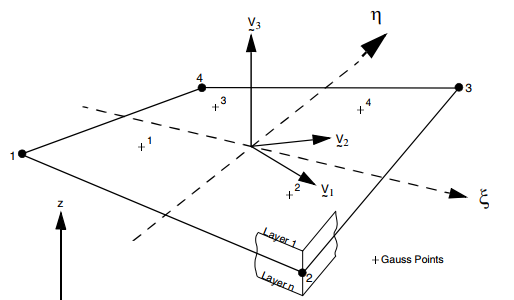
\includegraphics[width=0.5\textwidth]{figures/shell_element_schematic.png}
\caption{Schematic of the four-node bilinear thick-shell element (Marc Element~75) used for the MSC~Marc model: corner nodes 1--4, local director $v_3$ and in-plane axes $v_1$, $v_2$, curvilinear coordinates $\xi,\eta$, and through-thickness Gauss integration points across layers.}
\label{fig:shell-element}
\end{figure}

The two ends of the model are connected to the FE mesh through RBE2 rigid-body elements. RBE2 links can locally generate spurious over-stiffening and stress concentrations; this is considered acceptable here because stresses are not examined at the anchor points themselves (only the elbow region is of interest for stress results), so that the simpler RBE2 connection is preferred over an RBE3 connection.

% =============================================================================
\section{Elastic analysis and model calibration}
% =============================================================================

Before introducing plasticity, the two models are calibrated against one another on a purely elastic basis. Because the beam model represents elbow ovalisation only through the analytical flexibility factor $k$, whereas the shell model captures it directly through the finite-element discretisation, the anchor reaction moment (at the RBE2 master node) is used as the key comparison quantity, since it is highly sensitive to the overall flexibility of the system.

Table~\ref{tab:elastic-calib} reports the anchor reaction moment obtained with the beam model with and without the elbow flexibility factor, and with the shell model at increasing circumferential mesh densities.

\begin{table}[h]
\centering
\caption{Anchor reaction moment: beam model (with/without flexibility factor) versus shell FE model at increasing mesh density.}
\label{tab:elastic-calib}
\begin{tabular}{@{}lS@{}}
\toprule
\textbf{Model} & \textbf{Reaction moment [\si{N.m}]} \\
\midrule
NS beam model, without $k$-factor & 56702 \\
NS beam model, with $k$-factor ($k=10.1717$) & 39632 \\
MSC~Marc shell, 10 elements/circumference & 38260 \\
MSC~Marc shell, 20 elements/circumference & 39650 \\
MSC~Marc shell, 40 elements/circumference & 40180 \\
MSC~Marc shell, 80 elements/circumference & 40290 \\
\bottomrule
\end{tabular}
\end{table}

\begin{figure}[h]
\centering
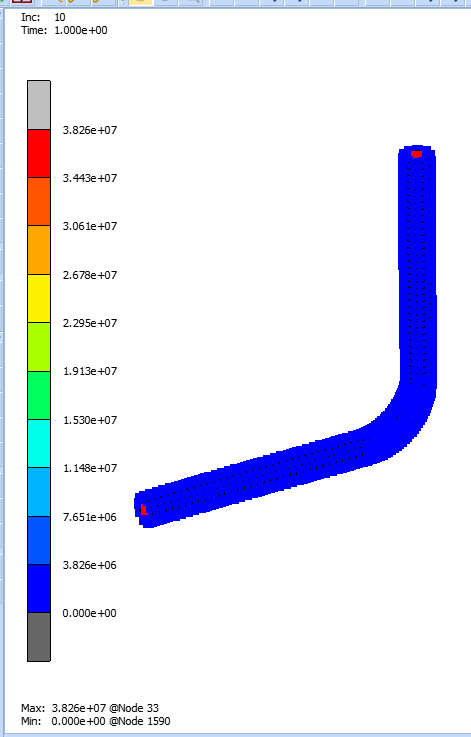
\includegraphics[width=0.42\textwidth]{figures/elastic_model_reaction.png}
\hfill
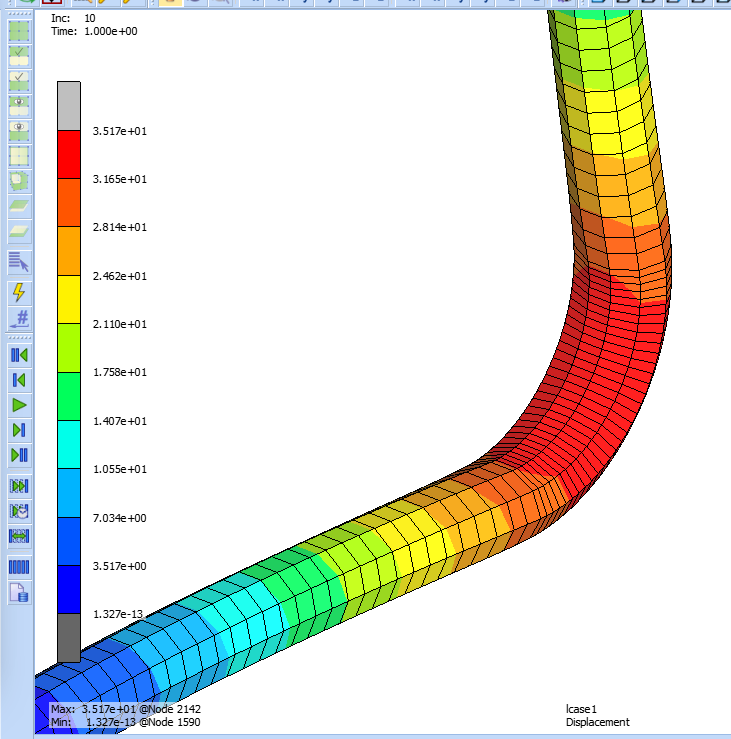
\includegraphics[width=0.42\textwidth]{figures/elastic_model_displacement.png}
\caption{MSC~Marc elastic shell model of the benchmark elbow. Left: overall geometry and elastic stress field, anchored at both ends. Right: deformed shape (magnified) coloured by displacement magnitude, showing the ovalisation-driven flexibility of the elbow region (maximum displacement \SI{35.17}{mm} at the free end, node 2142; anchor node 1590).}
\label{fig:elastic-model}
\end{figure}

The beam model without the elbow $k$-factor overestimates the system stiffness by about \SI{40}{\percent} relative to the converged shell solution, confirming the essential role of elbow ovalisation in the overall flexibility of the system. Once the analytical flexibility factor of Eq.~\eqref{eq:flexfactor} is introduced ($k=10.1717$), the beam-model reaction moment (\SI{39632}{N.m}) matches the shell result at a moderate mesh density (20 elements per circumference, \SI{39650}{N.m}) extremely well, confirming both the validity of the analytical flexibility factor and the adequacy of the beam-element representation for this geometry. As the shell mesh is further refined (40 and 80 elements per circumference), the reaction moment increases moderately further (\SI{40180}{} and \SI{40290}{N.m} respectively), indicating a degree of mesh sensitivity in the shell model that is revisited in Section~\ref{sec:discussion}. Large-deformation effects (ovalisation) are included in the shell analysis.

% =============================================================================
\section{Elasto-plastic analysis}
% =============================================================================

\subsection{Constitutive model}

The elasto-plastic shell analysis uses the Von Mises yield criterion with isotropic hardening, and the Ramberg--Osgood law of Eq.~\eqref{eq:RO} calibrated to 316L(N) at \SI{550}{\celsius} (RCC-MRx RB~A3.3S.451), with yielding onset defined at zero offset stress consistent with the code's convention. The shell mesh used for the elasto-plastic run (80 elements around the circumference) was checked beforehand for consistency with the elastic reference solution of Section~\ref{sec:benchmark}.

\subsection{Stress distribution and identification of the critical section}

The Von Mises stress distribution over the elbow shows a clearly identifiable ``weak link'' region (the section of maximum bending combined with ovalisation-amplified local stress), consistently located at the same position across all models, which is used as the reference cross-section for the abatement-coefficient comparison below.

\begin{figure}[h]
\centering
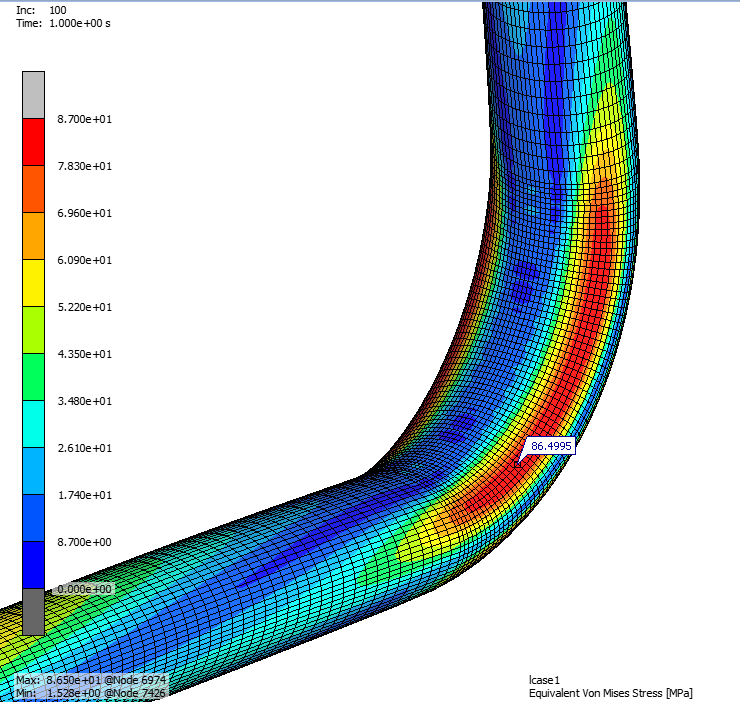
\includegraphics[width=0.6\textwidth]{figures/elastoplastic_vonmises_contour.png}
\caption{MSC~Marc elasto-plastic shell model (80 elements/circumference): equivalent Von~Mises stress distribution at the end of the thermal transient, showing the critical section at the elbow crown (maximum \SI{86.5}{MPa}, node 6974; minimum \SI{1.5}{MPa}, node 7426).}
\label{fig:vonmises}
\end{figure}

\subsection{Comparing the FE elasto-plastic and NS elastic-plus-code-rule approaches}

The RCC-MRx elastic route (RB~3651.1131) reduces the secondary (displacement-dependent) moment $m$ by the coefficient $g$ and combines the abated stress with the primary stress in the $\sigma_m+\sigma_b$ (P-type) damage check; equivalently, $g$ can be interpreted either as an abatement applied to the stresses (from the elastic/purely-secondary value down to the effective value) or as an abatement applied to the moments (from the elastic moment down to the effective moment). The natural benchmark question is then: \emph{how does the RCC-MRx-derived $g$ (and the associated $\sigma_m+\sigma_b$) compare with the coefficient and stress obtained from a full elasto-plastic FE reference calculation at the same critical section?}

Table~\ref{tab:g-comparison} reports this comparison.

\begin{table}[h]
\centering
\caption{Abatement coefficient $g$ and equivalent stress: RCC-MRx analytical route versus elasto-plastic FE reference.}
\label{tab:g-comparison}
\begin{tabular}{@{}lSS@{}}
\toprule
\textbf{Model / route} & \textbf{$g$} & \textbf{Stress [\si{MPa}]} \\
\midrule
Aspect Nuclear Pipe Stress, RCC-MRx (SMC1), $\sigma_m+\sigma_b$ & 0.323 & 66.5 \\
MSC~Marc elasto-plastic shell, Von Mises & 0.436 & 86.5 \\
\bottomrule
\end{tabular}
\end{table}

\begin{figure}[h]
\centering
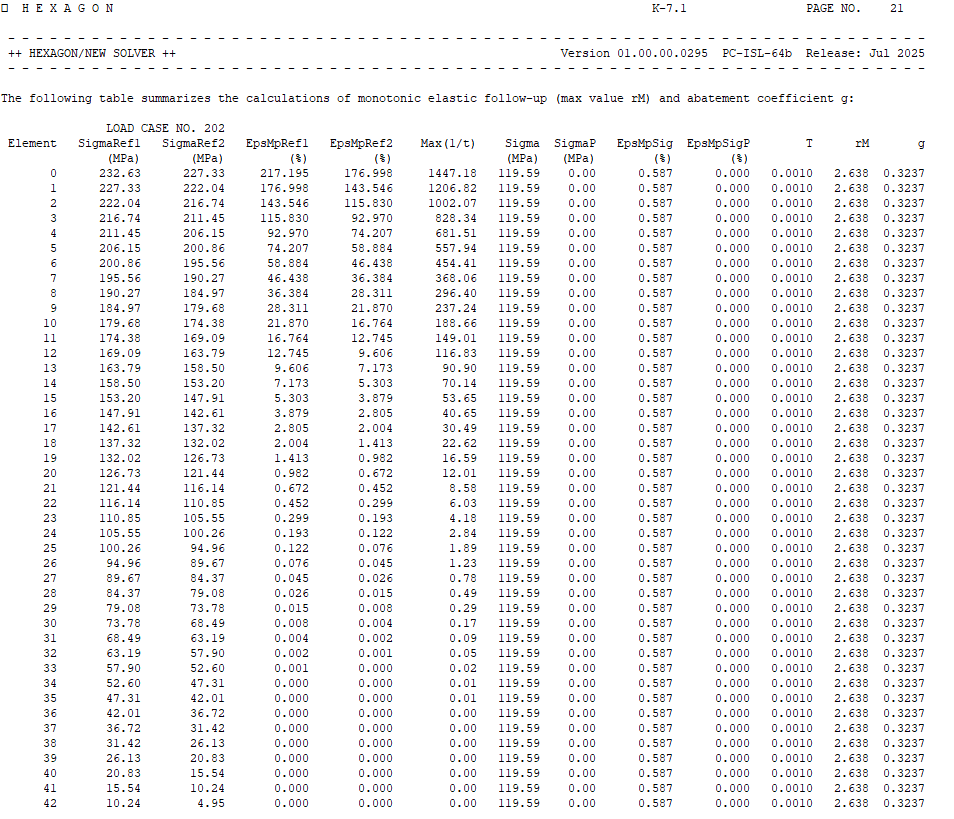
\includegraphics[width=0.85\textwidth]{figures/hexagon_benchmark_rM_g_table.png}
\caption{Actual production-code output (Aspect Nuclear Pipe Stress / HEXAGON NEW SOLVER, PC-ISL-64b) for the benchmark elbow under thermal load case LC~202: element-by-element elastic follow-up calculation, giving $T/t=r_M+1=2.638$ and $g=0.3237$ at the critical section, confirming the value reported in Table~\ref{tab:g-comparison}.}
\label{fig:hexagon-benchmark-table}
\end{figure}

\begin{figure}[h]
\centering
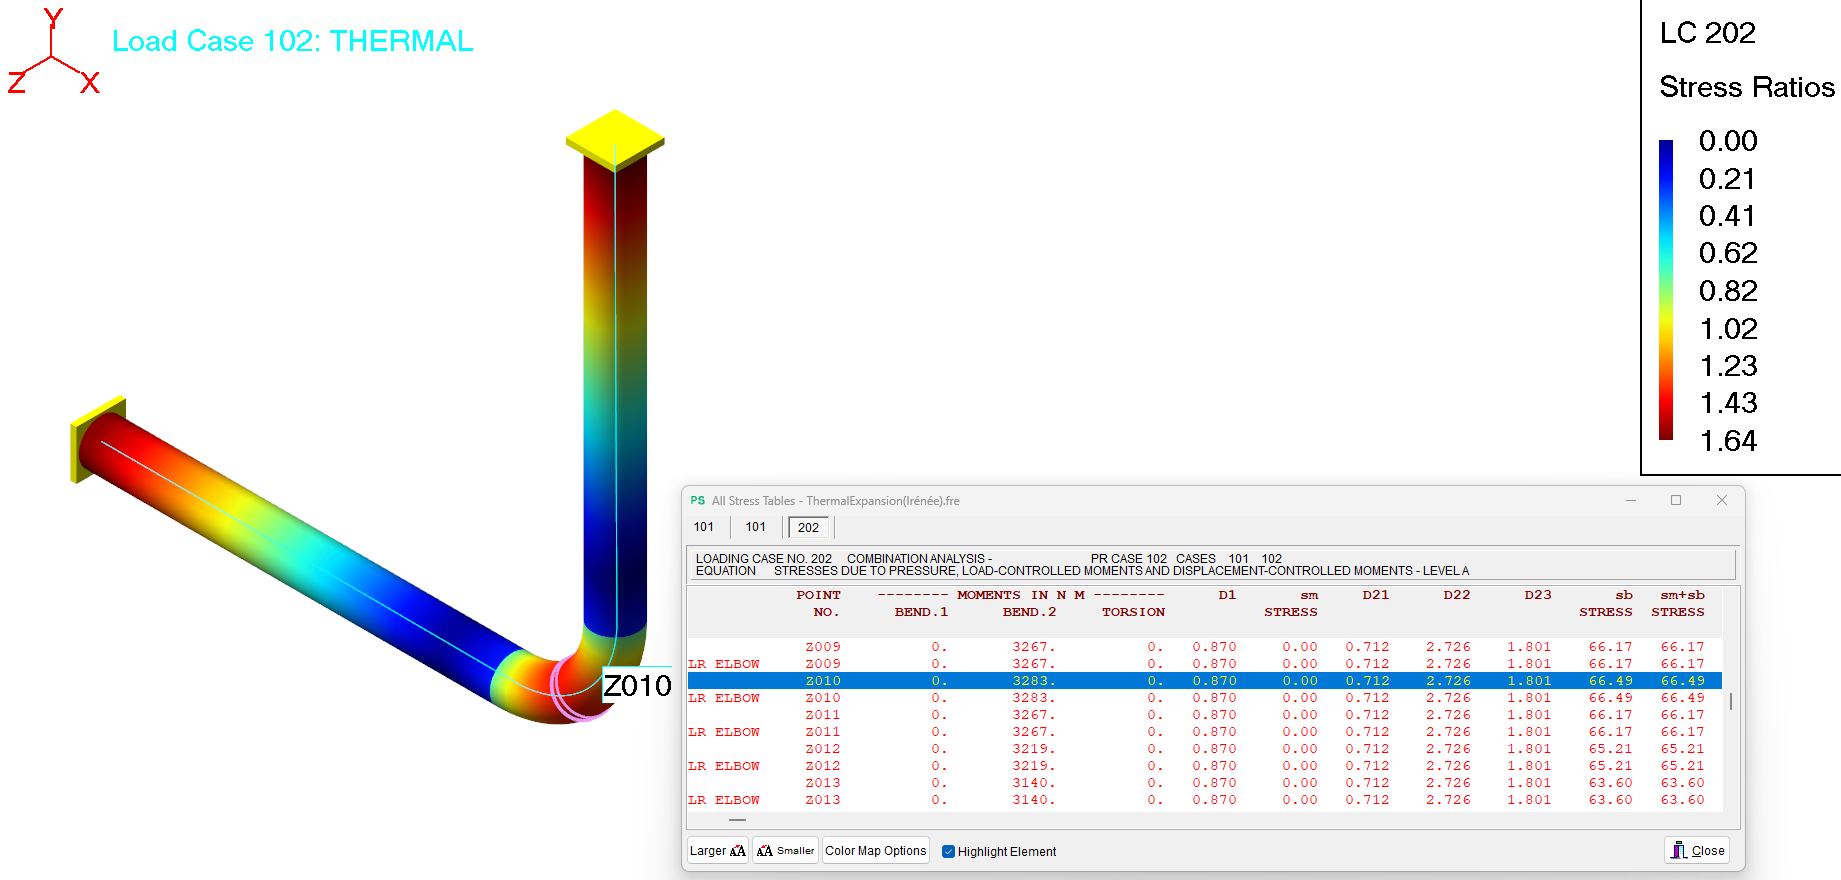
\includegraphics[width=0.75\textwidth]{figures/ns_solver_stress_table.png}
\caption{Aspect Nuclear Pipe Stress (NS solver) results for the thermal expansion load case (LC~202): stress-ratio colour map along the model and detailed stress table at the elbow points (Z009--Z013), giving $\sigma_m+\sigma_b=\SI{66.49}{MPa}$ at the critical point Z010, consistent with Table~\ref{tab:g-comparison}.}
\label{fig:ns-table}
\end{figure}

Two observations follow directly from Table~\ref{tab:g-comparison}:

\begin{enumerate}
\item \textbf{Observation 1:} the RCC-MRx abatement coefficient ($g=0.323$) is less conservative than the coefficient implied by the elasto-plastic FE reference ($g=0.436$).
\item \textbf{Observation 2:} the RCC-MRx primary-equivalent stress ($\sigma_m+\sigma_b = \SI{66.5}{MPa}$) is less conservative than the Von Mises stress of the reference elasto-plastic FE analysis (\SI{86.5}{MPa}).
\end{enumerate}

% =============================================================================
\section{Discussion: why is the RCC-MRx route less conservative?}
\label{sec:discussion}
% =============================================================================

\subsection{First explanation: primary-equivalent stress conversion}

RCC-MRx clause RB~3651.112 requires that, for load combinations governed by level-A criteria, the general primary membrane-plus-bending stress additionally satisfies
\begin{equation}
\overline{p_m+p_b} = B_1\,P\left[\frac{D_e}{2h_c}\right] + \left\langle B_2/Z,\,M\right\rangle \le 1.3\,S_m(\theta_m),
\label{eq:pmpb}
\end{equation}
i.e. the abated, displacement-dependent stress must ultimately be re-expressed and re-checked on the strictly primary allowable basis $1.3\,S_m(\theta_m)$, rather than on the CMS1 allowable $S^{*}$ of Eq.~\eqref{eq:CMS1} used to derive $g$ in Section~\ref{sec:rccmrx}. For the benchmark section considered here, $1.3\,S_m = \SI{100.1}{MPa}$ while $S^{*} = \SI{48.156}{MPa}$, so that the ratio
\begin{equation}
\frac{1.3\,S_m}{S^{*}} = \frac{100.1}{48.156} = 2.079
\end{equation}
is the conversion factor that must be applied when re-scaling the RCC-MRx abatement coefficient and stress from the $S^{*}$ (CMS1) basis onto the $1.3\,S_m$ (primary) basis:
\begin{equation}
g_{\mathrm{RCC\text{-}MRx}}^{\mathrm{rabat}} = g\cdot\frac{1.3\,S_m}{S^{*}} = 0.323\times 2.079 = 0.671, \qquad
(\sigma_m+\sigma_b)^{\mathrm{rabat}} = (\sigma_m+\sigma_b)\cdot\frac{1.3\,S_m}{S^{*}} = \SI{138.23}{MPa}.
\end{equation}
Once this conversion is applied, the RCC-MRx-based intensity of primary-type stress ($g^{\mathrm{rabat}}=0.671$, $(\sigma_m+\sigma_b)^{\mathrm{rabat}}=\SI{138.23}{MPa}$) becomes markedly \emph{more} conservative than the elasto-plastic FE reference ($g=0.436$, $\sigma_{\mathrm{VM}}=\SI{86.5}{MPa}$), reversing the apparent non-conservatism identified in Table~\ref{tab:g-comparison}. This confirms that the raw comparison of Table~\ref{tab:g-comparison} is not made on a consistent allowable-stress basis: $g$ and $\sigma_m+\sigma_b$ as computed under the CMS1 rule (RB~3651.1131, allowable $S^{*}$) are not directly comparable to a Von Mises stress checked against $1.3\,S_m$, and the code-mandated re-scaling of Eq.~\eqref{eq:pmpb} restores the expected conservatism of the analytical RCC-MRx route.

\subsection{Second explanation: mesh sensitivity of the reference solution}

An alternative (and complementary) explanation was sought by revisiting the mesh sensitivity noted already in Table~\ref{tab:elastic-calib}. When the elbow shell mesh used for the elasto-plastic MSC~Marc reference is examined for its impact on the RCC-MRx-style calculation of $g$ under the NS (Aspect Nuclear Pipe Stress) solver, the resulting $g$ converges, for a sufficiently refined mesh, towards the same value as the coefficient obtained directly from the elasto-plastic FE calculation ($g \approx 0.436$). In other words, once mesh convergence is properly achieved, the discrepancy between the RCC-MRx analytical route and the elasto-plastic reference is substantially reduced, without even invoking the primary-equivalent stress conversion of Section~\ref{sec:discussion}\,(first explanation). This indicates that at least part of the discrepancy originally observed in Table~\ref{tab:g-comparison} originates from an insufficiently refined shell mesh in the reference elasto-plastic model, rather than from an intrinsic shortcoming of the RCC-MRx $r_M/g$ formulation itself.

\begin{figure}[h]
\centering
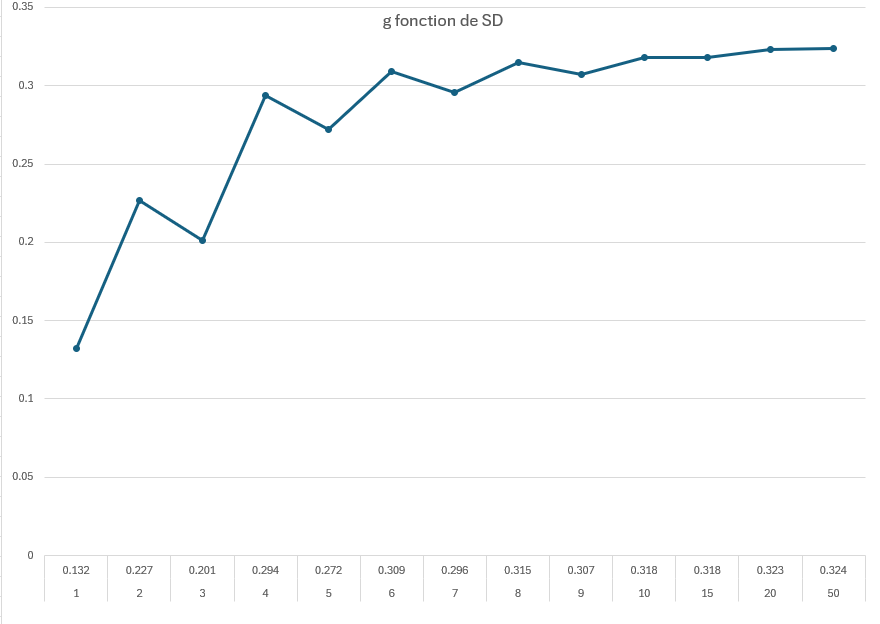
\includegraphics[width=0.65\textwidth]{figures/g_vs_mesh_convergence.png}
\caption{Convergence of the RCC-MRx abatement coefficient $g$ as a function of mesh refinement (shell subdivisions), confirming that $g$ tends towards the elasto-plastic FE reference value ($g\approx0.436$) as the mesh is refined.}
\label{fig:g-mesh-convergence}
\end{figure}

Both explanations are consistent with one another and are not mutually exclusive: the primary-equivalent stress conversion is a code-mandated, conservatism-restoring step that must always be applied; the mesh-sensitivity finding is a numerical-modelling caveat that must be controlled independently, regardless of which analytical route (RCC-MRx or direct elasto-plastic FE) is used.

\subsection{Additional validation: comparison across wall-thickness variants}

As a further, independent check, the RCC-MRx abatement coefficient $g$ obtained from the elasto-plastic FE reference ($g_{\mathrm{FEA}}$) was compared against the RCC-MRx analytical value ($g_{\mathrm{RCC\text{-}MRx}}$) on two additional model variants of the same benchmark, differing only in wall thickness (\SI{12}{mm} and \SI{15}{mm}), including large-strain and plasticity effects. In both cases, the RCC-MRx value bounds the FE-derived value, confirming the conservatism of the code-mandated coefficient across a range of section stiffnesses.

\begin{figure}[h]
\centering
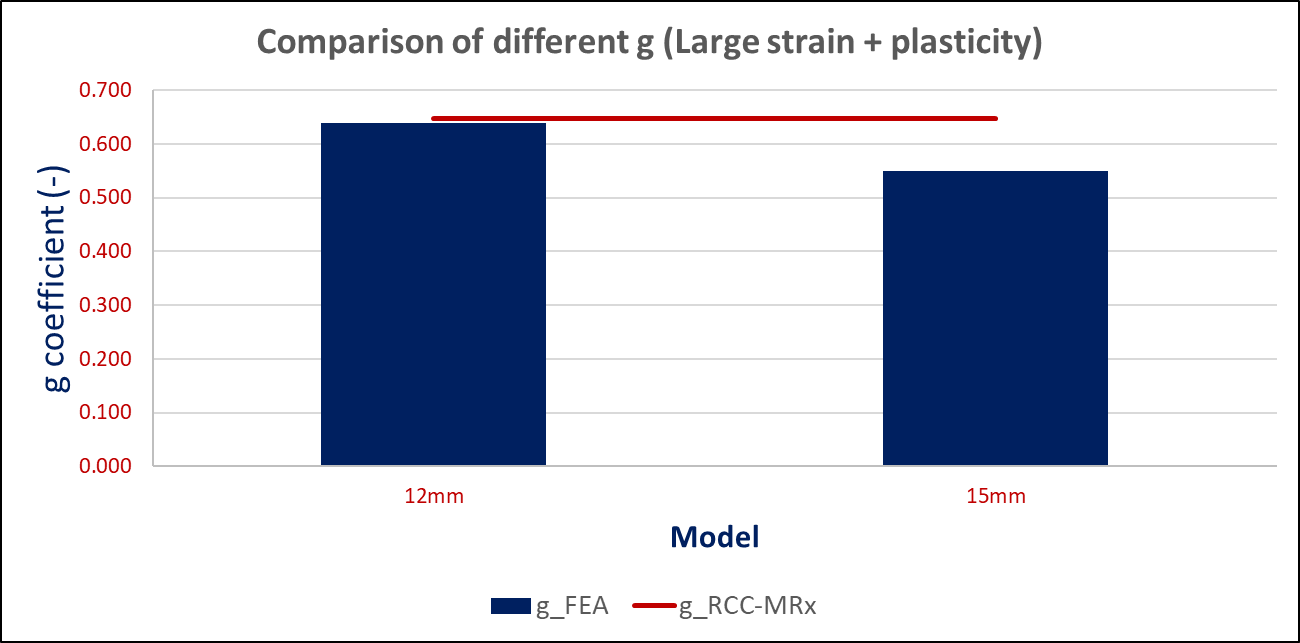
\includegraphics[width=0.65\textwidth]{figures/g_fea_vs_rccmrx_barchart.png}
\caption{Comparison of the abatement coefficient $g$ from a large-strain elasto-plastic FE calculation ($g_{\mathrm{FEA}}$) against the RCC-MRx analytical value ($g_{\mathrm{RCC\text{-}MRx}}$), for two wall-thickness variants (\SI{12}{mm} and \SI{15}{mm}) of the benchmark elbow. The RCC-MRx value remains conservative (equal to or above $g_{\mathrm{FEA}}$) in both cases.}
\label{fig:g-barchart}
\end{figure}

\subsection{Analytical validation on a cantilever with imposed end displacement}

To validate the production-code implementation of $r_M$ and $g$ independently of the elbow benchmark, a simple, closed-form case is considered: a straight cantilever beam of length $l$, clamped at one end, subjected to an imposed transverse displacement $\Delta u$ at the free end (Figure~\ref{fig:cantilever-sketch}).

\begin{figure}[h]
\centering
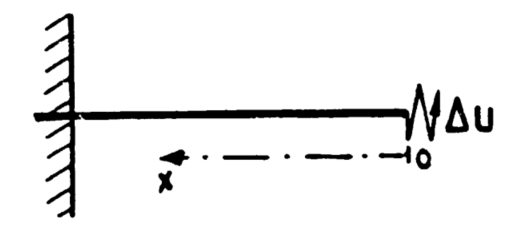
\includegraphics[width=0.5\textwidth]{figures/cantilever_sketch.png}
\caption{Schematic of the cantilever validation case: a beam of length $l$, clamped at $x=0$, with an imposed transverse displacement $\Delta u$ at the free end $x=l$.}
\label{fig:cantilever-sketch}
\end{figure}

For this configuration, the elastic reference stress is linear in $x$, $\sigma_{\mathrm{ref}}(x) = \omega\,x$ with $\omega = 0.79\,(3EI/l^{3})\,u/Z$, and the local resilience $1/t(x)$ follows directly from the Ramberg--Osgood plastic strain $\varepsilon_{M,p}$. Carrying out the integrals of Eq.~\eqref{eq:Tglobal} in closed form for this linear stress distribution gives the elastic follow-up factor as an explicit function of position,
\begin{equation}
r(x) \;=\; \frac{T}{t}-1 \;=\; \frac{1+2n_0}{3n_0}\left(\frac{x}{l}\right)^{\frac{1-n_0}{n_0}} - 1 ,
\label{eq:cantilever-rx}
\end{equation}
which is maximised at the clamped end ($x=0$, where $t\to\infty$, i.e.\ $\sigma_{\mathrm{ref}}\to 0$), giving the closed-form bound
\begin{equation}
r_{\max} \;=\; \frac{1-n_0}{3n_0} .
\label{eq:cantilever-rmax}
\end{equation}
For the benchmark material ($n_0=0.1125$), Eq.~\eqref{eq:cantilever-rmax} gives $r_{\max}=2.63$.

\begin{figure}[h]
\centering
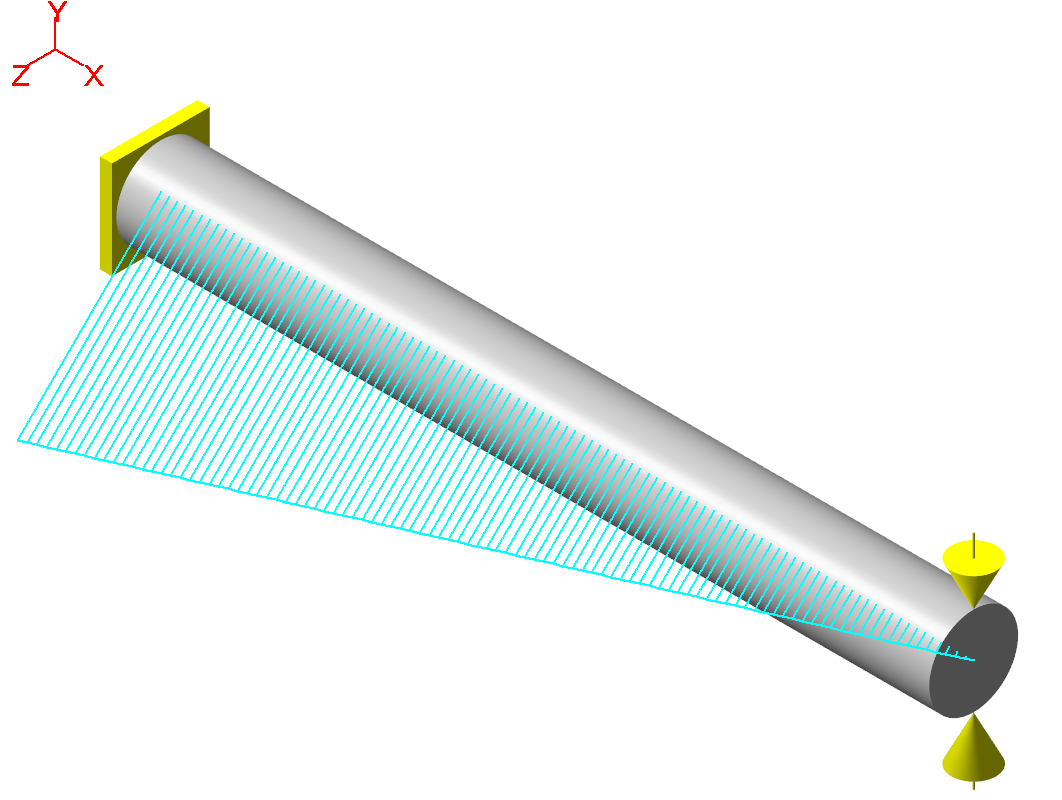
\includegraphics[width=0.75\textwidth]{figures/cantilever_3d_model.png}
\caption{Finite-element model of the cantilever validation case: clamped at one end (yellow anchor), imposed displacement enforced through a rigid link at the free end (yellow cones).}
\label{fig:cantilever-3d}
\end{figure}

\begin{figure}[h]
\centering
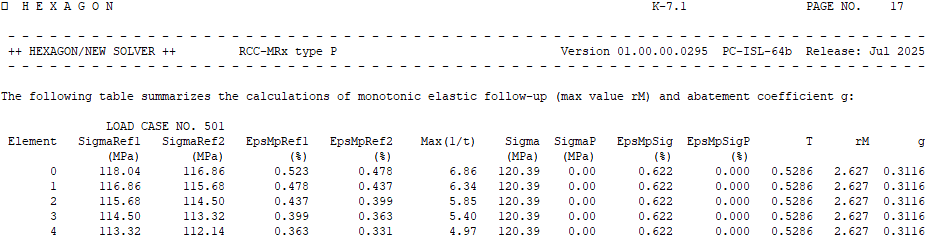
\includegraphics[width=0.85\textwidth]{figures/hexagon_cantilever_rM_g_table.png}
\caption{Production-code output (Aspect Nuclear Pipe Stress / HEXAGON NEW SOLVER, RCC-MRx type~P) for the cantilever validation case (LC~501): the code computes $T/t = r_M+1 = 2.627$, i.e.\ $r_M=1.627$, in close agreement with the closed-form bound $r_{\max}=2.63$ of Eq.~\eqref{eq:cantilever-rmax} at the clamped section, and $g=0.3116$.}
\label{fig:hexagon-cantilever-table}
\end{figure}

The close agreement between the closed-form analytical bound $r_{\max}=2.63$ and the production-code result ($T/t=2.627$) constitutes an independent, purely analytical validation of the code's implementation of the RCC-MRx elastic follow-up factor and abatement coefficient, on a case entirely decoupled from the elbow ovalisation and shell-modelling effects discussed above.

% =============================================================================
\section{Conclusions and perspectives}
% =============================================================================

\begin{enumerate}
\item Piping flexibility analysis methods have progressed considerably since the pioneering work of von~K\'arm\'an, Markl and Roche, from purely elastic beam theory to the modern treatment of elastic follow-up and elasto-plastic behaviour embodied in RCC-MRx.
\item Modern numerical tools bring gains in analysis turnaround time, but also introduce additional modelling complexity (mesh density, element formulation, boundary conditions) that must be carefully controlled.
\item The elastic benchmark shows good convergence between the beam-element piping code (Aspect Nuclear Pipe Stress) and the MSC~Marc shell model, at least for the resultant reaction forces and moments, once the analytical elbow flexibility factor is used consistently.
\item The results presented here highlight the importance of shell mesh density when computing the abatement coefficient $g$, both for the reference elasto-plastic solution and, indirectly, for any benchmark against it.
\item The present work has its own limitations, notably regarding the boundary conditions used (RBE2 connections) and the shell element formulation adopted; these should be kept in mind when interpreting the absolute stress values reported.
\item An open question remains whether the Ramberg--Osgood law, with a temperature-invariant hardening shape ($C_0$, $n_0$ constant for all temperatures), is adequate across the full range of operating temperatures relevant to high-temperature nuclear components.
\item Internal pressure was not included in the present study; extending the benchmark to pressurised conditions is a natural next step.
\end{enumerate}

% =============================================================================
\section*{Acknowledgements}
% =============================================================================
The authors thank the organisers of Pipe Stress Day 2026 (Lyon, France) for the opportunity to present this work.

Correspondence: \texttt{farid.tata@daes.pro}, \texttt{irenee.cornaton@octave.com}, \texttt{thuy.pham@octave.com}.

% =============================================================================
\appendix
\section{Sensitivity of the RCC-MRx abatement coefficient $g$ to mesh density}
% =============================================================================

As introduced in Section~\ref{sec:discussion}, the abatement coefficient $g$ computed under the RCC-MRx analytical route (Aspect Nuclear Pipe Stress, ``NS'' solver) was recomputed using anchor-reaction and local-flexibility data derived from shell models of increasing circumferential mesh density (10, 20, 40 and 80 elements per circumference, consistent with Table~\ref{tab:elastic-calib}). The resulting values of $g$ increase monotonically with mesh refinement and converge, at the finest mesh density considered, towards the value obtained directly from the elasto-plastic MSC~Marc reference calculation ($g\approx0.436$), confirming the mesh-sensitivity explanation of Section~\ref{sec:discussion}.

\section{Roland Roche's demonstration}
\label{app:roche}

This appendix reproduces, for completeness, the mathematical derivation of the elastic follow-up factor $r_M$ from the energy balance of a purely elastic finite-element analysis, following R.~Roche's original method \cite{Roche1987} as re-derived in an internal technical note accompanying the source presentation \cite{RochePipeStressNote}. This is the rigorous justification of Eqs.~\eqref{eq:rM}--\eqref{eq:Tglobal} used in Section~\ref{sec:rccmrx}.

\begin{figure}[h]
\centering
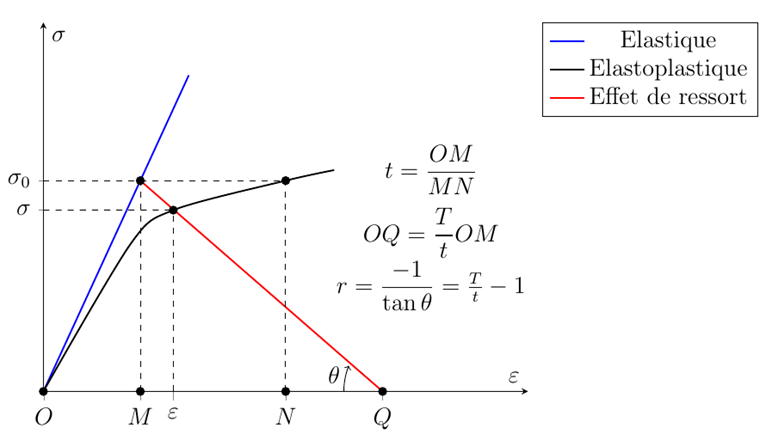
\includegraphics[width=0.65\textwidth]{figures/roche_graphical_construction.png}
\caption{Graphical construction of the elastic follow-up factor $r$ and local resilience $t$ from the elastic ($O$--$M$--$N$) and elasto-plastic ($O$--$\varepsilon$--$Q$) response curves at a given imposed strain: $t=OM/MN$ and the elastic-follow-up (``spring effect'') line through $(\varepsilon,\sigma)$ and $Q$ has slope $-\tan\theta = -1/(T/t-1)$.}
\label{fig:roche-graphical}
\end{figure}

\subsection{Standard variational development in a FE analysis}

The local equilibrium equation is $\sigma_{ij,j}+f_i=0$. Admitting a variational displacement field $\delta u$ applied at every material point, $\sigma_{ij,j}\delta u_i + f_i \delta u_i = 0$, and summing over the whole structure,
\begin{equation}
\iiint \sigma_{ij,j}\delta u_i \, dV + \iiint f_i \delta u_i \, dV = 0.
\end{equation}
Using $\sigma_{ij,j}\delta u_i = (\sigma_{ij}\delta u_i)_{,j} - \sigma_{ij}\delta u_{i,j}$ and the divergence theorem $\iiint(\sigma_{ij}\delta u_i)_{,j}\,dV = \iint \sigma_{ij}n_j\delta u_i\,dS$,
\begin{equation}
\iint \sigma_{ij}n_j\delta u_i\,dS - \iiint \sigma_{ij}\delta u_{i,j}\,dV + \iiint f_i\delta u_i\,dV = 0.
\end{equation}
With $\sigma_{ij}\delta u_{i,j} = \sigma_{ij}\tfrac12(\delta u_{i,j}+\delta u_{j,i}) = \sigma_{ij}\delta\varepsilon_{ij}$,
\begin{equation}
\iint \sigma_{ij}n_j\delta u_i\,dS - \iiint \sigma_{ij}\delta\varepsilon_{ij}\,dV + \iiint f_i\delta u_i\,dV = 0.
\label{eq:roche2}
\end{equation}
Assuming an external surface load $W_{\mathrm{ext}}=\int \sigma_{ij}n_j u_i\,dS$ with variational form $\delta W_{\mathrm{ext}} = \iint \delta\sigma_{ij}n_j u_i\,dS + \int \sigma_{ij}n_j\delta u_i\,dS$, and internal work $\delta W_{\mathrm{int}} = \delta\iiint \bar{\bar\sigma}:\bar{\bar\varepsilon}\,dV = \iiint \bar{\bar\sigma}:\delta\bar{\bar\varepsilon}\,dV + \iiint \delta\bar{\bar\sigma}:\bar{\bar\varepsilon}\,dV$, the principle of virtual work $\delta W_{\mathrm{int}}=\delta W_{\mathrm{ext}}$ gives
\begin{equation}
\iint \delta\sigma_{ij}n_j u_i\,dS + \iint \sigma_{ij}n_j\delta u_i\,dS = \iiint \sigma_{ij}\delta\varepsilon_{ij}\,dV + \iiint \delta\sigma_{ij}\varepsilon_{ij}\,dV.
\label{eq:roche3}
\end{equation}
From \eqref{eq:roche2}--\eqref{eq:roche3}, in the case $f_i=0$,
\begin{equation}
\iint \delta\sigma_{ij}n_j u_i\,dS = \iiint \delta\sigma_{ij}\varepsilon_{ij}\,dV.
\label{eq:roche4}
\end{equation}
Introducing a thermal (or other imposed-strain) contribution $\bar{\bar\epsilon}$, distinct from the mechanical strain $\bar{\bar\varepsilon}$,
\begin{equation}
\iiint \delta\bar{\bar\sigma}:\bar{\bar\varepsilon}\,dV = \iint \delta\bar{\bar\sigma}\,\vec n\,\vec u\,dS - \iiint \delta\bar{\bar\sigma}:\bar{\bar\epsilon}\,dV.
\label{eq:roche6}
\end{equation}
This is the working form used by Roche to derive $r_M$.

\subsection{Radially proportional elasto-plastic stress field}

Roche's method assumes that the elasto-plastic stress distribution remains, at every point, homogeneously proportional to the purely elastic solution, through a single scalar $\varphi$:
\begin{equation}
\bar{\bar\sigma} = \varphi\,\bar{\bar\sigma}_0.
\label{eq:roche7}
\end{equation}
Defining the equivalent (von Mises) stress and strain,
\begin{equation}
\varepsilon^{*} = \sqrt{\tfrac23 e_{ij}e_{ij}},\ e_{ij}=\varepsilon_{ij}-\tfrac13\varepsilon_{kk}\delta_{ij}; \qquad
\sigma^{*} = \sqrt{\tfrac32 s_{ij}s_{ij}},\ s_{ij}=\sigma_{ij}-\tfrac13\sigma_{kk}\delta_{ij},
\label{eq:roche89}
\end{equation}
Eq.~\eqref{eq:roche7} implies $\sigma^{*}=\varphi\,\sigma_0^{*}$. The plastic equivalent strain follows the Ramberg--Osgood law, Eq.~\eqref{eq:RO}:
\begin{equation}
\varepsilon^{*}(\sigma^{*}) = \varepsilon^{*}_{\mathrm{el}}(\sigma_0^{*}) + 0.01\left(\frac{\varphi\sigma_0^{*}}{C_0 R_{p0.2,\mathrm{moy}}}\right)^{1/n_0}
= \varphi\varepsilon_0^{*} + \phi\,\varepsilon_0^{p*}, \qquad \phi=\varphi^{1/n_0},
\label{eq:roche11}
\end{equation}
with $\varepsilon_0^{p*} = 0.01\left(\sigma_0^{*}/(C_0 R_{p0.2,\mathrm{moy}})\right)^{1/n_0}$.

\subsection{Energy balance}

Using Hooke's law $\varepsilon_{0ij} = \tfrac{1+\nu}{E}\sigma_{0ij}-\tfrac{\nu}{E}\sigma_{0kk}\delta_{ij}$, one obtains $e_{0ij} = \tfrac{1+\nu}{E}s_{0ij}$ and hence
\begin{equation}
\varepsilon_0^{*} = \frac{2}{3}\frac{1+\nu}{E}\sigma_0^{*}.
\label{eq:roche21}
\end{equation}
Combining Eqs.~\eqref{eq:roche11} and \eqref{eq:roche21} and defining the \emph{local resilience} $t=\varepsilon_0^{*}/\varepsilon_0^{p*}$, algebraic manipulation gives
\begin{equation}
\frac{3}{2(1+\nu)}\,\frac{E(\varepsilon^{*}-\varepsilon_0^{*})}{\sigma_0^{*}-\sigma^{*}} = \frac{T}{t}-1, \qquad
r_M = \frac{E(\varepsilon^{*}-\varepsilon_0^{*})}{\sigma_0^{*}-\sigma^{*}} \; \Rightarrow\; r_M = \frac{2(1+\nu)}{3}\left(\frac{T}{t}-1\right),
\label{eq:roche2223}
\end{equation}
where the \emph{global resilience} $T=\varepsilon_0^{*}/\varepsilon_0^{p*}$ is shown, by applying the energy balance of Eq.~\eqref{eq:roche6} to the purely elastic reference state and using Eqs.~\eqref{eq:roche7}--\eqref{eq:roche11},
\begin{equation}
(\varphi-1)\iiint \sigma_0^{*}\varepsilon_0^{*}\,dV + \phi\iiint \sigma_0^{*}\varepsilon_0^{p*}\,dV = 0
\;\Longrightarrow\;
T \equiv \frac{\iiint \sigma_0^{*}\varepsilon_0^{*}\,dV}{\iiint \sigma_0^{*}\varepsilon_0^{p*}\,dV} = \frac{\iiint {\sigma_0^{*}}^2\,dV}{\displaystyle\iiint \frac{{\sigma_0^{*}}^2}{t}\,dV},
\label{eq:roche1314}
\end{equation}
which, assuming a constant Young's modulus and constant equivalent stress within each piping section, reduces to the practical, section-integrated form used by RCC-MRx, Eq.~\eqref{eq:Tglobal}:
\begin{equation}
T = \frac{\int \sigma_0^{*2} A\,ds}{\displaystyle\int \frac{\sigma_0^{*2}A}{t}\,ds}.
\end{equation}

For steels ($\nu=0.3$), Eq.~\eqref{eq:roche2223} gives $r_M=0.867(T/t-1)$; the code's simplified, slightly more conservative form $r_M=T/t-1$ (Eq.~\eqref{eq:rM}) is obtained by taking $\tfrac{2(1+\nu)}{3}\approx1$, the associated 3-D correction being reintroduced separately as a 0.87 stress index on pressure and torsional-moment terms (Eq.~\eqref{eq:Tglobal}).

% =============================================================================
% References
% =============================================================================
\begin{thebibliography}{9}

\bibitem{VonKarman1911}
Th.~von K\'arm\'an,
\emph{\"{U}ber die Form\"{a}nderung d\"{u}nnwandiger Rohre, insbesondere federnder Ausgleichrohre},
Zeitschrift des Vereines deutscher Ingenieure, Vol.~55, pp.~1889--1895, 1911.

\bibitem{Markl1955}
A.R.C.~Markl,
\emph{Piping Flexibility Analysis},
Transactions of the ASME, Vol.~77, February 1955.

\bibitem{MillardRoche1981}
A.~Millard, R.~Roche,
\emph{Propagation of Ovalization along Straight Pipes and Elbows},
International Conference on Structural Mechanics in Reactor Technology (SMiRT), 1981.

\bibitem{Roche1987}
R.L.~Roche,
\emph{D\'etermination de la variation r\'eelle de d\'eformation \`a partir d'un calcul \'elastique (facteur $K_e$)},
1987.

\bibitem{RochePipeStressNote}
T.P.,
\emph{Mathematical demonstrations for Roland Roche method},
internal technical note, May 2026.

\bibitem{Flejou2024}
J.-L.~Fl\'ejou,
\emph{\'El\'ements ``exacts'' de poutres},
Code\_Aster reference manual, Fascicule r3.08, 2024.

\bibitem{NASAn1930}
NASA Technical Reports Server, \url{https://ntrs.nasa.gov/citations/19930081614}.

\bibitem{RCCMRx}
AFCEN, \emph{RCC-MRx: Design and Construction Rules for Mechanical Components of Nuclear Installations},
Sections RB~3643, RB~3651 and RB~A3.3S.451.

\end{thebibliography}

\end{document}
